%%-----------------------------------------------------------------------
% O argumento chapter=TITLE define que todos os títulos de capítulos
% saiam em caixa alta (maiúsculas). Se não quiser caixa alta, basta
% remover este argumento.
\documentclass[12pt,oneside,a4paper,chapter=TITLE,
			   english,brazil]{abntex2}


%%-----------------------------------------------------------------------
% Carregando a padronização para a capa, contra-capa e folha de
% assinaturas adotada pela UEPB
\usepackage{TCC_UEPB}

% Please add the following required packages to your document preamble:
\usepackage{multirow}
\usepackage[table,xcdraw]{xcolor}
\usepackage{colortbl} \usepackage[table,xcdraw]{xcolor}

%%-----------------------------------------------------------------------
% Pacotes básicos 
\usepackage{mathptmx}		% Usa a fonte Times New Roman
\usepackage[T1]{fontenc}	% Selecao de codigos de fonte.
\usepackage[utf8]{inputenc}	% Cod. do doc. (conversão autom. dos acentos)
\usepackage{lastpage}		% Usado pela Ficha catalográfica
\usepackage{indentfirst}	% Indenta o primeiro parágrafo de cada seção.
\usepackage{color}			% Controle das cores
\usepackage{graphicx}		% Inclusão de gráficos
\usepackage{microtype} 		% para melhorias de justificação
\usepackage{pdfpages}
\usepackage{supertabular}
\usepackage{float}
\usepackage{mdframed}
\usepackage{geometry}
\usepackage{multirow}
\bibliographystyle{abntex2-alf.bst} %Sobrenome em minusculo dos autores dentro de parenteses
\usepackage{colortbl}
\definecolor{lightgray}{gray}{0.9}


%%------------------------------------------------------------------------
% Pacotes adicionais, para definir ambientes para definição, teorema 
% e axioma. Outros ambientes podem ser definidos da mesma forma...
\usepackage{amssymb}     % qed
\usepackage{amsthm}      % Teoremas
\usepackage{amsmath}     % Para o ambiente align (alinhar equações)
\usepackage{thmtools}    % Front end para amsthm (\declaretheorem)


%%-----------------------------------------------------------------------
% Definição de ambientes para definição, teorema, etc...
\declaretheorem[style=definition,name=Definição,qed=\textemdash]{definicao}
\declaretheorem[style=plain,name=Teorema,qed=\textnormal{\textemdash}]{teorema}
\declaretheorem[style=plain,name=Axioma,qed=\textnormal{\textemdash}]{axioma}
\declaretheorem[style=plain,name=Lema,qed=\textnormal{\textemdash}]{lema}
\usepackage{pdfpages}
\usepackage{float}

%%------------------------------------------------------------------------
% Pacotes de citações
\usepackage[brazilian,hyperpageref]{backref} % Página citada na bibliog.
\usepackage[alf]{abntex2cite}				 % Citações padrão ABNT



%%-----------------------------------------------------------------------
%% CONFIGURAÇÕES DE PACOTES
%%-----------------------------------------------------------------------


%%-----------------------------------------------------------------------
% Configurações do pacote backref Usado sem a opção hyperpageref
% de backref
\renewcommand{\backrefpagesname}{Citado na(s) página(s):~}
% Texto padrão antes do número das páginas
\renewcommand{\backref}{}   % Define os textos da citação
\renewcommand*{\backrefalt}[4]{
	\ifcase #1 %
	Nenhuma citação no texto.%
	\or
	Citado na página #2.%
	\else
	Citado #1 vezes nas páginas #2.%
	\fi}%


%%----------------------------------------------------------------------
% Configurações de aparência do PDF final
\makeatletter
\hypersetup{     % informações do PDF
	pdftitle={\@title}, 
	pdfauthor={\@author},
	pdfsubject={\imprimirpreambulo},
	colorlinks=true,   % false: box links; true: color links
	linkcolor=black,   % color of internal links
	citecolor=black,   % color of links to bibliography
	filecolor=black,   % color of file links
	urlcolor=black,    % color of url links
	bookmarksdepth=4
}
\makeatother


%%------------------------------------------------------------------
% Cria uma nova série (de símbolos) para footnotes
\newcounter{savefootnote}
\newcounter{symfootnote}
\newcommand{\symfootnote}[1]{%
	\setcounter{savefootnote}{\value{footnote}}%
	\setcounter{footnote}{\value{symfootnote}}%
	\ifnum\value{footnote}>8\setcounter{footnote}{0}\fi%
	\let\oldthefootnote=\thefootnote%
	\renewcommand{\thefootnote}{\fnsymbol{footnote}}%
	\footnote{#1}%
	\let\thefootnote=\oldthefootnote%
	\setcounter{symfootnote}{\value{footnote}}%
	\setcounter{footnote}{\value{savefootnote}}%
}


%Informações
\titulo{PROGNITIVE: Promovendo Habilidades Cognitivas de Programação para Alunos do Ensino Médio, Técnico e Profissionalizante da Região de Patos-PB.} 
\autor{Mikaelle Oliveira Santos Gomes} 
\local{Patos - PB}
\data{2025}


\makeindex
\begin{document}

\frenchspacing 
\pretextual
\imprimircapa

%Ficha catalográfica
%\begin{fichacatalografica}
%\includepdf{figuras/Ficha-Catalografica.pdf}
%\end{fichacatalografica}
\setcounter{page}{2}

%Folha de aprovação

% Inserir folha de aprovação
\setlength{\ABNTEXsignwidth}{8cm}    


%Elementos Textuais
\textual
\pagestyle{simple}
\aliaspagestyle{chapter}{simple}

\chapter{APRESENTAÇÃO DOS DADOS CADASTRAIS}

\begin{itemize}
    \item \textbf{Título do Projeto/Programa/ Curso/Evento:} PROGNITIVE: Promovendo Habilidades Cognitivas de Programação para Alunos do Ensino Médio, Técnico e Profissionalizante da Região de Patos-PB.
    \item \textbf{Área Temática:} Educação
    \item \textbf{Linha Programática:} Educação e Cidadania
    \item \textbf{Nº de Cadastro/ registro do Projeto na PROEX:} 
\end{itemize}
\chapter{IDENTIFICAÇÃO DOS PARTICIPANTES}

\section{Coordenação}

\begin{itemize}
    \item \textbf{Nome:} Dra. Mikaelle Oliveira Santos Gomes
    \item \textbf{E-mail:} mikaelleoliveira@servidor.uepb.edu.br
    \item \textbf{Centro:} Centro de Ciências Exatas e Sociais Aplicadas
    \item \textbf{Departamento de Lotação:} -
    \item \textbf{Curso:} Computação
    \item \textbf{Contato:} 83-99123-8620
\end{itemize}

\section{Professores Colaboradores}

\vspace{1em}

\begin{itemize}
    \item \textbf{Nome:} Dr. Jucelio Soares dos Santos
    \item \textbf{E-mail:} jucelio@servidor.uepb.edu.br
    \item \textbf{Centro:} Centro de Ciências Exatas e Sociais Aplicadas
    \item \textbf{Departamento de Lotação:} -
    \item \textbf{Curso:} Computação
    \item \textbf{Contato:} 83-99394-0726 
\end{itemize}

\section{Alunos Participantes}

\begin{table}[H]
\caption{Número de Alunos Monitores e Professores Envolvidos no Projeto.}
\centering
\begin{tabular}{|l|r|}
\hline
\textbf{Descrição}               & \textbf{Quantidade} \\ \hline
Número total de alunos voluntários & 4                 \\ \hline
Número total de alunos bolsitas      & 1                   \\ \hline
Número total de alunos participantes      & 5                   \\ \hline
\end{tabular}
\label{num-alunos-professores}
\end{table}
\vspace{1em}

\begin{itemize}
    \item \textbf{Nome:} Luanny Kelly de Almeida Leitão 
    \item \textbf{E-mail:} luanny.leitao@aluno.uepb.edu.br
    \item \textbf{Centro:} Centro de Ciências Exatas e Sociais Aplicadas
    \item \textbf{Departamento de Lotação:} -
    \item \textbf{Curso:} Computação
    \item \textbf{Contato:} 83 99617-2593
    \item \textbf{Bolsista:} Sim
\end{itemize}

\vspace{1em}

\begin{itemize}
    \item \textbf{Nome:} André Vinícius Barros Macambira
    \item \textbf{E-mail:} andre.macambira@aluno.uepb.edu.br
    \item \textbf{Centro:} Centro de Ciências Exatas e Sociais Aplicadas
    \item \textbf{Departamento de Lotação:} -
    \item \textbf{Curso:} Computação
    \item \textbf{Contato:} 83 98624-2005
    \item \textbf{Bolsista:} Não 
\end{itemize}

\vspace{1em}

\begin{itemize}
    \item \textbf{Nome:} Jhefferson Kauã Dias de Araujo
    \item \textbf{E-mail:} jhefferson.araujo@aluno.uepb.edu.br
    \item \textbf{Centro:} Centro de Ciências Exatas e Sociais Aplicadas
    \item \textbf{Departamento de Lotação:} -
    \item \textbf{Curso:} Computação
    \item \textbf{Contato:} 83 99992-0910
    \item \textbf{Bolsista:} Não 
\end{itemize}

\vspace{1em}

\begin{itemize}
    \item \textbf{Nome:} Myllena de Sousa Medeiros
    \item \textbf{E-mail:} myllena.sousa@aluno.uepb.edu.br
    \item \textbf{Centro:} Centro de Ciências Exatas e Sociais Aplicadas
    \item \textbf{Departamento de Lotação:} -
    \item \textbf{Curso:} Computação
    \item \textbf{Contato:} 83 98658-6571
    \item \textbf{Bolsista:} Não 
\end{itemize}

\vspace{1em}

\begin{itemize}
    \item \textbf{Nome:} Vinícius França de Oliveira Sousa
    \item \textbf{E-mail:} vinicius.franca@aluno.uepb.edu.br
    \item \textbf{Centro:} Centro de Ciências Exatas e Sociais Aplicadas
    \item \textbf{Departamento de Lotação:} -
    \item \textbf{Curso:} Computação
    \item \textbf{Contato:} 83 99695-6202
    \item \textbf{Bolsista:} Não 
\end{itemize}
\chapter{INTRODUÇÃO}

O projeto em questão tem como principal objetivo fomentar o aprendizado de programação e robótica entre estudantes do Ensino Médio, por meio de abordagens educacionais inovadoras e metodologias ativas que tornem o processo de ensino mais envolvente e significativo, além de divulgar o curso de ciência da Computação do Câmpus VII da UEPB. 

A partir de ações diversificadas e contextualizadas, busca-se proporcionar uma vivência formativa que una teoria e prática de forma equilibrada e eficiente.

As atividades tiveram início com aulas de lógica de programação, seguida de aulas utilizando a linguagem Java, com ênfase em conceitos de Orientação a Objetos, diretamente aplicados à robótica educacional. Essa integração favorece o desenvolvimento de competências técnicas sólidas, preparando os alunos para enfrentar tanto desafios computacionais quanto práticos, típicos da robótica moderna.

Para reforçar o conteúdo abordado, foram propostos exercícios de fixação que estimulam a aprendizagem ativa, promovendo o raciocínio lógico e o pensamento algorítmico. Essa estratégia contribui para uma assimilação mais eficaz dos conceitos, ao mesmo tempo em que fortalece a autonomia e a capacidade de resolução de problemas dos estudantes.

Durante a execução do projeto, ofereceu-se acompanhamento individualizado, com suporte contínuo na resolução de dúvidas e na realização das atividades práticas. Essa atenção personalizada permitiu respeitar o ritmo de aprendizagem de cada participante, tornando o processo mais inclusivo e eficiente.

Um dos recursos tecnológicos explorados foi o Road Runner, ferramenta que converte o ambiente da arena em um plano cartesiano, otimizando a movimentação do robô durante a fase autônoma da competição. 

O projeto também visa preparar os alunos para a participação na FTC (FIRST Tech Challenge), uma renomada competição nacional e internacional de robótica. Essa etapa final agrega valor à experiência educacional, ao incentivar a aplicação prática do conhecimento adquirido, fortalecer o espírito de equipe e inspirar os estudantes a seguirem carreiras nas áreas de Ciência, Tecnologia, Engenharia e Matemática (STEM).

Com uma proposta estruturada e abrangente, o projeto se destaca por oferecer uma formação prática, desafiadora e motivadora, contribuindo diretamente para preparação de jovens frente às exigências do mundo tecnológico contemporâneo.

 
\chapter{OBJETIVOS}

A educação em Ciência da Computação e Robótica tem um papel estratégico na formação de estudantes capazes de lidar com os desafios tecnológicos do século XXI. Nesse contexto, o projeto "Prognitive"  se apresenta como uma resposta proativa às necessidades educacionais contemporâneas, com a proposta de ir além do ensino tradicional, promovendo um aprendizado prático, personalizado e interdisciplinar. Neste capítulo, serão apresentados os objetivos traçados pelo projeto e as principais ações desenvolvidas para sua concretização.

\section{Objetivos Propostos e Discussões das Ações Desenvolvidas}

O projeto "Prognitive" estabelece como objetivos centrais:

\begin{itemize}
    \item Ministrar aulas de programação com a linguagem Java, fundamentadas nos princípios da Orientação a Objetos, integrando esses conhecimentos aos conceitos da robótica educacional, com o intuito de desenvolver competências técnicas e estruturadas em programação;
    \item Estimular a aprendizagem ativa por meio de exercícios de fixação, favorecendo o desenvolvimento do raciocínio lógico e da construção de algoritmos, aspectos essenciais na formação em computação;
    \item Oferecer acompanhamento individualizado aos alunos, promovendo o esclarecimento de dúvidas e o apoio na execução das atividades, assegurando um processo de aprendizagem mais eficaz e ajustado às particularidades de cada estudante;
    \item Inserir e aplicar a ferramenta Road Runner, convertendo a arena em um plano cartesiano, o que possibilita um controle mais preciso do robô na fase autônoma, inclusive em trajetórias não lineares, ampliando as habilidades de programação e estratégias de movimentação;
    \item Preparar os discentes para competir na First Tech Challenge (FTC), competição nacional e internacional de robótica educacional, oferecendo base técnica e científica, experiência prática e incentivo ao trabalho em equipe e à resolução de problemas;
    \item Estimular o interesse dos alunos pelas áreas de Ciência, Tecnologia, Engenharia e Matemática (STEM), contribuindo para a formação de futuros profissionais nessas áreas estratégicas para o desenvolvimento tecnológico.
\end{itemize}

Diversas ações foram implementadas em diferentes cenários, utilizando abordagens dinâmicas e focadas no engajamento estudantil:

\begin{itemize}
    \item Realização de aulas práticas de programação com a linguagem Java, aliadas à robótica com foco em conceitos de Orientação a Objetos;
    \item Proposição de exercícios de fixação com desafios práticos, reforçando o conteúdo e promovendo o pensamento computacional;
    \item Atendimento contínuo aos alunos, com suporte direto na resolução de atividades e dúvidas durante as práticas;
    \item Introdução e aplicação da ferramenta Road Runner, permitindo que os alunos programem trajetórias com base em coordenadas cartesianas e compreendam os efeitos de suas escolhas na movimentação real do robô;
    \item Preparação para participação na FTC, com atividades direcionadas para treino da competição e desenvolver estratégias em equipe.
    \item Prestação de mentoria na construção científica do portfólio da equipe, contribuindo com orientações quanto à organização, redação técnica e apresentação das atividades desenvolvidas, fortalecendo a identidade e a comunicação do projeto.
\end{itemize}

\section{Objetivos Alcançados}

Os objetivos delineados pelo projeto "Prognitive" foram atingidos de forma expressiva e produtiva. Todas as ações planejadas foram executadas com êxito, proporcionando aos alunos um ambiente propício ao desenvolvimento técnico em programação e robótica. O suporte individualizado permitiu que cada estudante avançasse conforme seu próprio ritmo, enfrentando e superando dificuldades com segurança e motivação. A utilização da ferramenta \textit{Road Runner} e o treinamento voltado para a FTC contribuíram significativamente para a consolidação das habilidades práticas e do pensamento estratégico. Como fruto desse esforço, a equipe de Robótica Legonautas participou da Temporada 2023/2024 da \textit{FIRST Tech Challenge}, conquistando o título de Vice-Campeões na Arena e sendo premiados como Aliança Capitã Finalista. Na temporada 2024/2025, a equipe também chegou às etapas finais na arena do campeonato. Além disso, observou-se um notável aumento no interesse dos alunos por áreas STEM, demonstrando que o projeto cumpriu com êxito seu propósito de inspirar e formar jovens para os desafios tecnológicos do presente e do futuro.

\chapter{METODOLOGIA, ESTRATÉGIAS DE AÇÃO, MATERIAL E MÉTODOS}

Neste capítulo, são apresentados a metodologia adotada, as estratégias de ação implementadas, bem como os materiais e métodos utilizados no desenvolvimento do projeto "Prognitive". A integração entre teoria e prática é destacada como elemento essencial do processo, assegurando que os conhecimentos adquiridos fossem contextualizados e aplicados de forma significativa.

Para garantir a eficácia das atividades realizadas, foram implementadas diversas estratégias metodológicas, incluindo:

\begin{itemize}
    \item Aulas expositivas, com ênfase nos conceitos fundamentais de programação, robótica e áreas correlatas, a fim de fornecer uma base teórica sólida aos participantes;
    \item Atividades práticas \textit{hands-on}\footnote{\textit{"Hands-on"} refere-se à experiência prática e direta, em que os participantes lidam ativamente com o conteúdo por meio da experimentação e execução de tarefas. Isso favorece a internalização do conhecimento \cite{graafstra2007hands}.}, utilizando kits de robótica, simuladores e plataformas digitais para a aplicação dos conhecimentos;
    \item Estudos de caso, por meio dos quais os alunos analisaram problemas reais e propuseram soluções baseadas nos conteúdos aprendidos;
    \item Debates em grupo, estimulando a reflexão crítica, o raciocínio argumentativo e o trabalho em equipe;
    \item Resolução de problemas práticos nas áreas de lógica, programação e automação, incentivando a criatividade e a eficiência;
    \item Uso de recursos digitais interativos, como ambientes virtuais de aprendizagem, vídeos, quizzes, tutoriais e jogos educacionais;
    \item Acompanhamento individualizado dos alunos, com orientação contínua, escuta ativa, esclarecimento de dúvidas e devolutivas personalizadas;
    \item Oficinas temáticas e dinâmicas de grupo com foco em criatividade, liderança, pensamento computacional e ética na tecnologia.
\end{itemize}

Essas estratégias foram fundamentadas em teorias pedagógicas sólidas, como a teoria da aprendizagem significativa de Ausubel \cite{ausubel1982aprendizagem, junior2023olhar}, a abordagem socioconstrutivista de Vygotsky \cite{vygotsky1988aprendizagem, paixao2019aprendizagem, cantuaria2023importancia}, e em metodologias ativas contemporâneas de ensino-aprendizagem \cite{kripka2020ensino}, como o \textit{Design Thinking} Educacional, que favorece a empatia, ideação, prototipação e solução de problemas reais. Todo o processo foi adaptado ao perfil dos participantes, considerando seus níveis de conhecimento, motivações, interesses e dificuldades.

Durante a execução do projeto, diversos materiais, ferramentas e recursos foram utilizados para apoiar e potencializar o processo de aprendizagem. Destacam-se:

\begin{itemize}
    \item \textbf{Kits de robótica:} Conjuntos de componentes eletrônicos e mecânicos para montagem de protótipos robóticos;
    \item \textbf{Computadores e dispositivos móveis:} Utilizados para programação, simulação, pesquisa e uso de softwares educacionais;
    \item \textbf{Material impresso:} Apostilas, manuais, guias práticos e roteiros de atividades, que complementaram o conteúdo digital;
    \item \textbf{Recursos de comunicação:} E-mails, fóruns online, plataformas de reuniões e chats de apoio;
    \item \textbf{Simuladores virtuais:} Plataformas como simuladores de linguagem de programação;
    \item \textbf{Softwares educacionais:} Ambientes como Visual Studio Code e plataformas gamificadas;
    \item \textbf{Ambientes físicos preparados:} Salas de aula com acesso à internet, projetores, quadros interativos, mobiliário móvel e climatização;
    \item \textbf{Agenda e cronograma:} Planejamento semanal com datas, temas, atividades e avaliações;
\end{itemize}

Em relação aos métodos pedagógicos, buscou-se adotar abordagens centradas no aluno, com foco na aprendizagem ativa e significativa. Foram utilizados:

\begin{itemize}
    \item \textbf{Aprendizagem baseada em problemas (PBL):} Método centrado em situações-problema para promover autonomia, pesquisa e tomada de decisão;
    \item \textbf{Ensino colaborativo:} Organização de equipes com papéis definidos, promovendo cooperação, comunicação e corresponsabilidade;
    \item \textbf{Aprendizagem ativa:} Metodologias que envolvem diretamente os participantes, como debates, projetos e dinâmicas reflexivas;
    \item \textbf{Feedback construtivo:} Avaliações formativas com devolutivas detalhadas e orientações para melhoria contínua;
    \item \textbf{Gamificação:} Uso de elementos de jogos (desafios, pontuações, recompensas) para aumentar o engajamento;
    \item \textbf{Rodas de conversa e autoavaliação:} Espaços de fala e escuta, nos quais os alunos refletiam sobre o próprio processo de aprendizagem;
    \item \textbf{Aprendizagem baseada em projetos (PjBL):} Desenvolvimento de soluções tecnológicas com etapas de planejamento, execução e apresentação final;
    \item \textbf{Mentorias e tutoria entre pares:} Acompanhamento individual e colaboração entre alunos mais experientes e iniciantes.
\end{itemize}

A diversidade e complementaridade dos métodos adotados contribuiu significativamente para uma experiência de aprendizado rica, contextualizada e alinhada às exigências das competições de robótica e ao desenvolvimento de competências STEM. O uso integrado de diferentes abordagens pedagógicas, associado aos recursos didáticos e tecnológicos, assegurou o cumprimento dos objetivos educacionais propostos e o desenvolvimento integral dos participantes.

\chapter{ETAPAS DO PROJETO}

O projeto foi organizado em etapas estratégicas e sequenciais, cada uma com objetivos bem definidos e ações planejadas para alcançá-los de forma eficiente. A seguir, descrevem-se essas etapas em detalhes:

\begin{itemize}
    \item \textbf{Levantamento de Necessidades:} A fase inicial consistiu na identificação das principais demandas e dificuldades enfrentadas pelos estudantes no processo de aprendizagem de programação e robótica. Foram conduzidas entrevistas, questionários diagnósticos e observações em sala para mapear os conhecimentos prévios, os interesses dos participantes e os recursos disponíveis na escola;
    
    \item \textbf{Planejamento e Estruturação:} Com base nas informações levantadas, foi realizada a construção do plano de ação do projeto. Nessa etapa, definiram-se os objetivos gerais e específicos, a carga horária, a sequência didática dos conteúdos, as metodologias a serem aplicadas, os critérios de avaliação, o cronograma e os recursos materiais, humanos e tecnológicos necessários para a execução das atividades;
    
    \item \textbf{Desenvolvimento de Conteúdo:} Foram elaborados materiais didáticos interativos voltados para o ensino de programação e robótica com foco no desenvolvimento de competências STEM. Os conteúdos foram adaptados ao público-alvo, incluindo slides, vídeos, apostilas digitais, roteiros de atividades práticas, simuladores online, jogos educativos e protótipos experimentais. Também foram preparados desafios inspirados em competições de robótica;
    
    \item \textbf{Implementação das Ações:} Iniciou-se a execução das aulas teóricas e práticas, seguindo a metodologia ativa. Os estudantes participaram de oficinas, desafios de programação, construção de robôs e resolução de problemas, estimulando o raciocínio lógico, a criatividade e o trabalho em equipe. Também foram realizadas mentorias técnicas e rodas de conversa sobre carreira científica e tecnológica;
    
    \item \textbf{Acompanhamento e Avaliação:} O progresso dos participantes foi monitorado de forma contínua, por meio da observação direta, autoavaliações, resolução de exercícios, devolutivas qualitativas e desafios avaliativos. As avaliações formativas e somativas permitiram identificar avanços cognitivos, engajamento, desenvolvimento de habilidades práticas e dificuldades pontuais, possibilitando ajustes nas estratégias ao longo do percurso;
    
    \item \textbf{Análise de Resultados:} Com a conclusão das atividades, foi realizada uma avaliação global dos resultados obtidos. A análise envolveu a comparação entre os objetivos iniciais e os resultados alcançados, destacando indicadores como melhoria no desempenho, aumento do interesse pelas áreas de ciência e tecnologia e engajamento nas dinâmicas propostas. A equipe também refletiu sobre os desafios enfrentados e as boas práticas identificadas;
    
    \item \textbf{Documentação e Relatório Final:} Todas as fases do projeto foram devidamente registradas, resultando na elaboração de um relatório técnico-científico final. Esse documento sistematiza as ações realizadas, os resultados obtidos, os instrumentos utilizados, os aprendizados coletivos e as recomendações para a replicação e aprimoramento de projetos futuros com escopo semelhante.
\end{itemize}

\chapter{IDENTIFICAÇÃO DAS AÇÕES DESENVOLVIDAS}

Para garantir o cumprimento dos objetivos do projeto Prognitive, foram realizadas diversas ações ao longo de sua execução. As atividades foram conduzidas semanalmente, no Laboratório de Informática da Escola Dionísio Marques de Almeida. A seguir, apresentam-se as datas e os conteúdos abordados em cada encontro, organizados de forma progressiva para preparar os estudantes tanto no domínio da programação quanto na atuação em robótica competitiva, com foco em Java e no uso de tecnologias como Road Runner.

\vspace{1em}

\textbf{Momento I – Introdução ã Lógica de Programação}

\begin{itemize}
    \item 15/08/24: Apresentação do projeto e introdução ao pensamento computacional
    \item 19/08/24: Introdução ã Lógica de Programação
    \item 22/08/24: Introdução à Linguagem Java
    \item 29/08/24:  Tipos de dados, constantes e variáveis
\end{itemize}

\textbf{Momento II – Fundamentos de Programação em Java}

\begin{itemize}
    \item 05/09/24: Entrada e saída de dados com a classe Scanner
    \item 12/09/24: Correção coletiva de atividades práticas
    \item 19/09/24: Comandos de seleção e comandos de repetição (if e else, while e for)
    \item 26/09/24: Vetores, matrizes e manipulação de strings
    \item 03/10/24: Funções, Procedimentos e Recursividade
    \item 10/10/24: Registros e Enumerações
\end{itemize}

\textbf{Momento III – Programação Orientada a Objetos}

\begin{itemize}
    \item 17/10/24: Introdução à Programação Orientada a Objetos: 
    \item 24/10/24: Classes, Objetos, Atributos e Métodos
    \item 31/10/24: Objetos e Construtores
    \item 07/11/24: Composição e Agregação 
    \item 14/11/24: Encapsulamento e Abstração
    \item 21/11/24: Herança e Polimorfismo
    \item 28/11/24: Coleções em Java
    \item 05/12/24: Tratamento e Lançamento de Exceções 
    \item 12/12/24: Classes Abstratas e Interfaces
\end{itemize}

\textbf{Momento IV – Robótica com Java e Programação de Trajetórias}

\begin{itemize}
    \item 02/01/25: Manipulação de motores, sensores e servos com a FTC SDK
    \item 09/01/25: Programação de controle manual (TeleOp) no contexto do robô FTC
    \item 16/01/25: Introdução ao Road Runner e noções básicas de movimentação autônoma
    \item 23/01/25: Programação de trajetórias com Road Runner: conceitos e funções principais
    \item 30/01/25: Ajustes de PID, precisão e tempo nos movimentos autônomos
    \item 06/02/25: Integração entre modos autônomo e manual; estratégias para a competição
    \item 13/02/25: Simulação de partidas e revisão geral dos códigos com foco na FTC
    \item 20/02/25: Preparação final e revisão para a competição
\end{itemize}

Essas ações foram planejadas e executadas de forma a proporcionar aos participantes do projeto uma progressão gradual no aprendizado, abordando desde os conceitos básicos da linguagem de programação Java até tópicos mais avançados relacionados à Programação Orientada a Objetos. Cada encontro (Fig. \ref{fig:4}, Fig. \ref{fig:5} e Fig. \ref{fig:6})  foi estruturado para fornecer uma base sólida de conhecimento e habilidades aos alunos, preparando-os para enfrentar desafios mais complexos no campo da computação e da robótica.

\begin{figure}[H]
    \centering
    \includegraphics[scale=0.22]{imagens/imagem11.png}
    \caption{Início das ações no Centro de Atividades Dionízio Marques de Almeida - Patos - PB.}
    \label{fig:4}
\end{figure}

\begin{figure}[H]
    \centering
    \includegraphics[scale=0.22]{imagens/imagem3.jpeg}
    \caption{Aula sobre Comandos de Decisão utilizando a linguagem Java.}
    \label{fig:5}
\end{figure}

\begin{figure}[H]
    \centering
    \includegraphics[scale=0.22]{imagens/imagem2.jpeg}
    \caption{Aula sobre Herança a linguagem Java.}
    \label{fig:6}
\end{figure}

\chapter{DURAÇÃO DO PROJETO}

O projeto Prognitive teve uma duração total de um ano. Durante esse período, diversas ações e atividades de extensão foram realizadas com o objetivo de promover o aprendizado de programação e robótica, além de engajar os participantes em competições nacionais de tecnologia, como a FIRST Tech Challenge (FTC).

A execução do projeto foi organizada em módulos educacionais que contemplaram desde a introdução à lógica de programação e à linguagem Java até tópicos avançados de programação orientada a objetos. Essas aulas, que ocorreram semanalmente, foram complementadas por workshops e atividades práticas, visando garantir que os participantes não apenas compreendessem os conceitos teóricos, mas também tivessem a oportunidade de aplicar o conhecimento adquirido.

Além das aulas e atividades de ensino, o projeto se dedicou à capacitação prática por meio de oficinas de robótica, focando principalmente no desenvolvimento e programação de robôs. A participação em competições de robótica foi uma das partes mais importantes do projeto, pois proporcionou aos alunos a oportunidade de aplicar as habilidades adquiridas em um ambiente competitivo. A preparação para a competição nacional e internacional foi intensiva, abrangendo desde a montagem e configuração de robôs até o desenvolvimento de algoritmos avançados de controle de movimentos, como o uso do Road Runner para trajetórias autônomas.

Ao longo do projeto, foram realizados momentos de análise e discussão dos resultados das competições, com a finalidade de identificar pontos de melhoria e possibilitar um feedback construtivo.

Em termos de impacto, o projeto "Prognitive" contribuiu significativamente para o desenvolvimento educacional, social e profissional dos participantes. A inclusão de alunos de diferentes níveis de conhecimento em computação e robótica propiciou a democratização do acesso à educação tecnológica de qualidade, além de fomentar o interesse pelas áreas de ciência e inovação.

 O projeto "Prognitive" se mostrou uma experiência enriquecedora tanto para os participantes quanto para a comunidade, com resultados positivos no desenvolvimento de competências técnicas e interpessoais.

\chapter{IDENTIFICAÇÃO DA COMUNIDADE PARTICIPANTE NA AÇÃO DE EXTENSÃO}

As ações extensionistas do projeto foram direcionadas principalmente na escola Dionízio Marques de Almeida, visando atingir um público diversificado e promover o acesso à educação em ciência da computação e robótica.

Durante a execução do projeto, foram estabelecidos os seguintes convênios, contratos e acordos de cooperação:

\begin{itemize}
\item \textbf{Convênios celebrados:}
\begin{itemize}
\item Instituições públicas federais: 0
\item Instituições públicas estaduais: 0
\item Instituições públicas municipais: 0
\item Movimentos Sociais Organizados: 0
\end{itemize}
\item \textbf{Contratos firmados:}
\begin{itemize}
    \item Instituições públicas federais: 0
    \item Instituições públicas estaduais: 0
    \item Instituições públicas municipais: 0
    \item Movimentos Sociais Organizados: 0
\end{itemize}

\item \textbf{Acordos de cooperação estabelecidos:}
\begin{itemize}
    \item Instituições públicas federais: 0
    \item Instituições públicas estaduais: 0
    \item Instituições públicas municipais: 0
    \item Movimentos Sociais Organizados: 0
\end{itemize}

\end{itemize}

Além disso, registrou-se o número de pessoas externas à UPEB (Universidade Pública Estadual da Baixada) participantes/atendidas pelo projeto, curso ou evento:

\begin{enumerate}
\item \textbf{Da Comunidade:}
\begin{itemize}
\item Quantidade: 40
\end{itemize}

\item \textbf{Como Colaborador(a):}
\begin{itemize}
    \item Quantidade: 2
\end{itemize}

\item \textbf{Carga horária:}
\begin{itemize}
    \item Semanal: 4
    \item Mensal: 20
    \item Total: 360
\end{itemize}
\end{enumerate}

Este registro inclui tanto a participação/atendimento durante as atividades desenvolvidas, planejamento das ações, como também aquelas realizadas por meio da prestação de serviços.

\chapter{LOCAL DE REALIZAÇÃO}

O projeto "Prognitive" foi implementado integralmente na Escola Dionísio Marques de Almeida (DMA), situada na cidade de Patos - PB, com o objetivo de atender aos alunos do Ensino Médio desta instituição, visando uma formação sólida nas áreas de programação e robótica.

A escolha da escola como local de realização do projeto foi estratégica , sendo um dos principais fatores a infraestrutura disponível para o desenvolvimento de atividades práticas. A escola já possuía kits de robótica, o que facilitou a implementação das atividades propostas no projeto. Além disso, a presença de um laboratório de informática bem equipado foi um diferencial crucial, pois permitiu que os alunos utilizassem recursos tecnológicos avançados para aprofundar seus conhecimentos em programação e robótica.

O laboratório de informática foi fundamental para criar um ambiente interativo e dinâmico, essencial para o aprendizado prático de programação. Com computadores modernos e acesso contínuo à internet, os alunos puderam desenvolver suas habilidades através de pesquisas online, prática em linguagens de programação e acesso a materiais educacionais complementares. Esse espaço se tornou um centro de aprendizagem, onde os alunos puderam, além de programar, colaborar em projetos, simular cenários e resolver problemas complexos de maneira colaborativa.

Ademais, a combinação do laboratório de informática com os kits de robótica proporcionou aos alunos uma experiência de aprendizagem prática e envolvente. As aulas foram estruturadas de forma a integrar a construção de robôs físicos com a programação de suas trajetórias e comportamentos, permitindo que os estudantes não só aprendessem a lógica de programação, mas também a aplicassem em um ambiente real, com resultados tangíveis. Essa abordagem prática estimulou a criatividade e a resolução de problemas de maneira inovadora, alinhada às metodologias ativas de ensino.

Portanto, a escolha do local de realização do projeto "Prognitive" foi um fator determinante para o sucesso da iniciativa. A infraestrutura tecnológica disponível, somada ao comprometimento da escola em apoiar o desenvolvimento educacional dos alunos, possibilitou a implementação de um ensino inovador, eficaz e alinhado com as demandas atuais de formação em ciência e tecnologia. O projeto contribuiu significativamente para a promoção do aprendizado em programação e robótica, preparando os alunos para os desafios do futuro.

\chapter{RESULTADOS E CONTRIBUIÇÕES DO PROJETO À COMUNIDADE}

O capítulo de Resultados e Contribuições do Projeto à Comunidade apresenta uma análise abrangente dos impactos e benefícios gerados pela execução do "Prognitive" em sua comunidade-alvo. Ao longo do período de implementação, uma série de resultados positivos foi observada, evidenciando a eficácia e relevância das iniciativas propostas.

Um dos resultados mais notáveis foi o aumento significativo do interesse dos alunos pelas áreas de Computação e STEM. Essa crescente motivação foi percebida tanto na participação ativa dos estudantes nas atividades do projeto quanto em seu engajamento em buscar conhecimento adicional fora do ambiente escolar. Esse incremento no interesse demonstra o impacto direto do projeto na promoção da educação e formação de futuros profissionais em áreas tecnológicas.

Além disso, os participantes do projeto apresentaram uma melhoria substancial em suas habilidades de programação e raciocínio lógico. Isso se refletiu não apenas em avaliações internas e externas, onde os alunos obtiveram resultados expressivos, mas também em sua capacidade aprimorada de resolver problemas de forma eficiente e criativa. Essa habilidade é crucial não apenas para o sucesso acadêmico, mas também para a preparação dos jovens para os desafios do mercado de trabalho.

Outro aspecto relevante dos resultados obtidos foi a participação destacada dos alunos em competições de robótica e feiras de ciências  (Fig. \ref{fig:1} e Fig.\ref{fig:3}). Nessas ocasiões, os estudantes puderam aplicar os seus conhecimentos adquiridos no projeto de forma prática, demonstrando suas habilidades para a comunidade e contribuindo para a visibilidade da escola e do projeto no cenário local, regional e nacional. Nesse sentido, destaca-se a participação da equipe de robótica Legonautas na Competição FTC, Temporada 2023/2024 e 2024/2025 da FTC e foram Vice Campeões na Arena, ganhando o prêmio de Aliança Capitã Finalista. 

\begin{figure}[H]
    \centering
    \includegraphics[scale=0.8]{imagens/imagem9.jpeg}
    \caption{Participação dos Alunos atendidos pelo projeto na Competição Nacional da FTC em Brasília.}
    \label{fig:1}
\end{figure}

Além dos resultados individuais dos participantes, o "Prognitive" também trouxe contribuições significativas para a comunidade em geral. Em primeiro lugar, o projeto estimulou o desenvolvimento tecnológico local, ao formar uma nova geração de estudantes capacitados em áreas como programação e robótica. Esses jovens talentosos têm o potencial de contribuir significativamente para a inovação e o crescimento econômico da região.

O projeto fortaleceu o vínculo entre a escola e a comunidade, ao envolver pais, responsáveis e outros membros da sociedade nas atividades do projeto. Essa colaboração entre diferentes atores sociais é essencial para promover uma educação de qualidade e para preparar os jovens para os desafios do século XXI.

O "Prognitive" proporcionou oportunidades para os alunos desenvolverem habilidades de liderança e trabalho em equipe. A participação em projetos de programação e robótica exigiu que os estudantes trabalhassem juntos para alcançar objetivos comuns, preparando-os para desafios futuros no ambiente de trabalho (Fig. \ref{fig:3}). 

Além de aprimorar as habilidades técnicas em programação e robótica, o projeto também proporcionou aos alunos oportunidades para o desenvolvimento de habilidades de liderança, trabalho em equipe e resolução de problemas em grupo. A participação em competições de robótica e no desenvolvimento de projetos exigiu uma intensa colaboração entre os estudantes para o desenvolvimento de soluções criativas em conjunto.

\begin{figure}[H]
    \centering
    \includegraphics[scale=0.6]{imagens/imagem8.jpeg}
    \caption{Preparação do Robô para Competição utilizando Road Runner.}
    \label{fig:3}
\end{figure}

\begin{figure}[H]
    \centering
    \includegraphics[scale=0.22]{imagens/imagem 20.jpg}
    \caption{Prêmio de Aliança Finalista - FTC.}
    \label{fig:4}
\end{figure}

Por fim, o projeto teve um impacto significativo e duradouro no desenvolvimento do pensamento crítico e criativo dos alunos e da comunidade. Ao serem desafiados a resolver problemas complexos e desenvolver soluções inovadoras através da programação e da robótica, os participantes aprimoraram suas habilidades de análise, tomada de decisões e resolução de problemas. Essas competências são fundamentais não só para a carreira profissional, mas também para a formação de cidadãos engajados e capazes de contribuir positivamente para a sociedade.

\chapter{PRODUÇÕES CIENTÍFICAS RESULTANTES DO PROJETO DE EXTENSÃO}

Durante o período inicial de execução do "Prognitive", o foco principal esteve na implementação das atividades e na interação com a comunidade. À medida que o projeto avançou, conseguimos alcançar novos patamares, com a produção das primeiras publicações científicas que analisam e documentam os resultados obtidos e os impactos gerados.

O primeiro artigo científico gerado pelo projeto, intitulado "Contributions of the PROGNITIVE Project to the Development of Programming and Robotics Skills in High School", marca um ponto de inflexão significativo na jornada do "Prognitive". Este trabalho analisa o impacto do projeto no desenvolvimento de habilidades de programação e robótica em estudantes do ensino médio, destacando a maneira como a iniciativa tem impulsionado a aprendizagem prática nessas áreas.

\begin{figure}[H]
    \centering
    \caption{Apresentação do artigo "Contributions of the PROGNITIVE Project to the Development of Programming and Robotics Skills in High School" durante o VI Sercomp. }
    \includegraphics[scale=0.20]{imagens/imagem18.jpeg}
\end{figure}

\begin{figure}[H]
    \centering
    \caption{Apresentação do artigo científico sobre o Projeto Prognitive, destacando as contribuições para o ensino de programação e robótica no ensino médio.}
    \includegraphics[scale=0.18]{imagens/imagem21.jpeg.jpg}
    \includegraphics[scale=0.18]{imagens/imagem19.jpeg.jpg}
\end{figure}


Com o sucesso da primeira publicação, planejamos expandir nossas ações para criar novas produções científicas, ampliando a abrangência do projeto com as seguintes iniciativas:
\begin{itemize}
    \item Publicação de artigos científicos que explorem aspectos específicos do "Prognitive", com foco em áreas como ensino de programação, uso de robótica como ferramenta pedagógica.
    \item Produção de livros e manuais para documentar as metodologias e práticas que se mostraram bem-sucedidas ao longo do projeto.
    \item Desenvolvimento de softwares e jogos educativos, como ferramentas para estimular a aprendizagem interativa e engajante nas áreas de programação e robótica.
\end{itemize}



\chapter{EVENTOS DE EXTENSÃO REALIZADOS}

Infelizmente, não foi possível realizar eventos de extensão durante o período do projeto. No entanto,esperamos poder organizar uma variedade de eventos no futuro, tais como seminários, fóruns, congressos, semanas temáticas, palestras, dinâmicas, oficinas, entre outros, para promover ainda mais o engajamento com a comunidade e disseminar conhecimento sobre programação e robótica.

Porém, durante a execução do projeto, diversas atividades de extensão foram realizadas para promover o aprendizado em computação e compartilhar os resultados obtidos. Dessas atividades, destaca-se a oferta do workshop "Desenvolvimento de Competências para Competições de Robótica com Java". Sendo uma das iniciativas de maior relevância, foi projetado para fornecer aos participantes as habilidades necessárias para se destacarem em competições de robótica utilizando a linguagem de programação Java.

\begin{figure}[H]
    \centering
    \caption{Capa da oferta do workshop "Desenvolvimento de Competências para Competições de Robótica com Java" durante o VI Sercomp.}
    \includegraphics[scale=0.2]{imagens/imagem17.jpg}
\end{figure}

\vspace{2em}

Durante o evento do VI SERCOMP (Congresso Sertanejoo de Computação), os participantes aprenderam os fundamentos da programação em Java e como aplicar esses conhecimentos na programação de robôs para competições de alto nível, como as competições da FTC (First Tech Challenge). Através de uma abordagem prática e focada no desenvolvimento de habilidades específicas, o workshop teve grande impacto.

\begin{figure}[H]
    \centering
    \caption{Participantes do workshop "Desenvolvimento de Competências para Competições de Robótica com Java" em atividade.}
    \includegraphics[scale=0.2]{imagens/imagem16.jpg}
\end{figure}

Além do workshop mencionado, outras atividades de extensão foram realizadas, promovendo o aprendizado em computação e fortalecendo os vínculos entre o projeto e a comunidade acadêmica.

Outro exemplo dessas atividades foi a oferta da Jornada de Atualização em Computação "Introdução à Orientação a Objetos em Java: Conceitos e Exemplos Práticos", realizada durante o VI Semana Zero do Curso de Computação. Neste evento, os participantes tiveram a oportunidade de aprender os princípios fundamentais da programação orientada a objetos, uma base essencial para o desenvolvimento de aplicações em Java.

\begin{figure}[H]
    \centering
    \caption{Oferta da Jornada de Atualização em Computação "Introdução à Orientação a Objetos em Java: Conceitos e Exemplos Práticos" durante o VI Semana Zero do Curso de Computação.}
    \includegraphics[scale=0.18]{imagens/imagem15.jpeg}
\end{figure}

Outro destaque foi o minicurso "Programação em Java: Introdução aos Fundamentos e Sintaxe", oferecido durante o I Congresso de Fluência entre Ensino, Tecnologia e Gestão. Esse minicurso forneceu uma introdução prática à linguagem Java, abordando desde a sintaxe básica até os primeiros conceitos de programação.

\begin{figure}[H]
    \centering
    \caption{Oferta do Minicurso "Programação em Java: Introdução aos fundamentos e sintaxe" durante o I Congresso de Fluência entre Ensino, Tecnologia e Gestão.}
    \includegraphics[scale=0.4]{imagens/imagem14.jpeg}
\end{figure}

Adicionalmente, participamos da Mostra de Extensão durante a VII Semana Zero do Curso de Computação, onde os resultados do projeto foram apresentados. Neste evento, tivemos a oportunidade de compartilhar com a comunidade acadêmica os impactos do "Prognitive", os objetivos atingidos e os planos para as próximas fases do projeto.

\begin{figure}[H]
    \centering
    \caption{Participação na Mostra de Extensão para apresentar os Resultados do Projeto durante a VII Semana Zero do Curso de Computação.}
    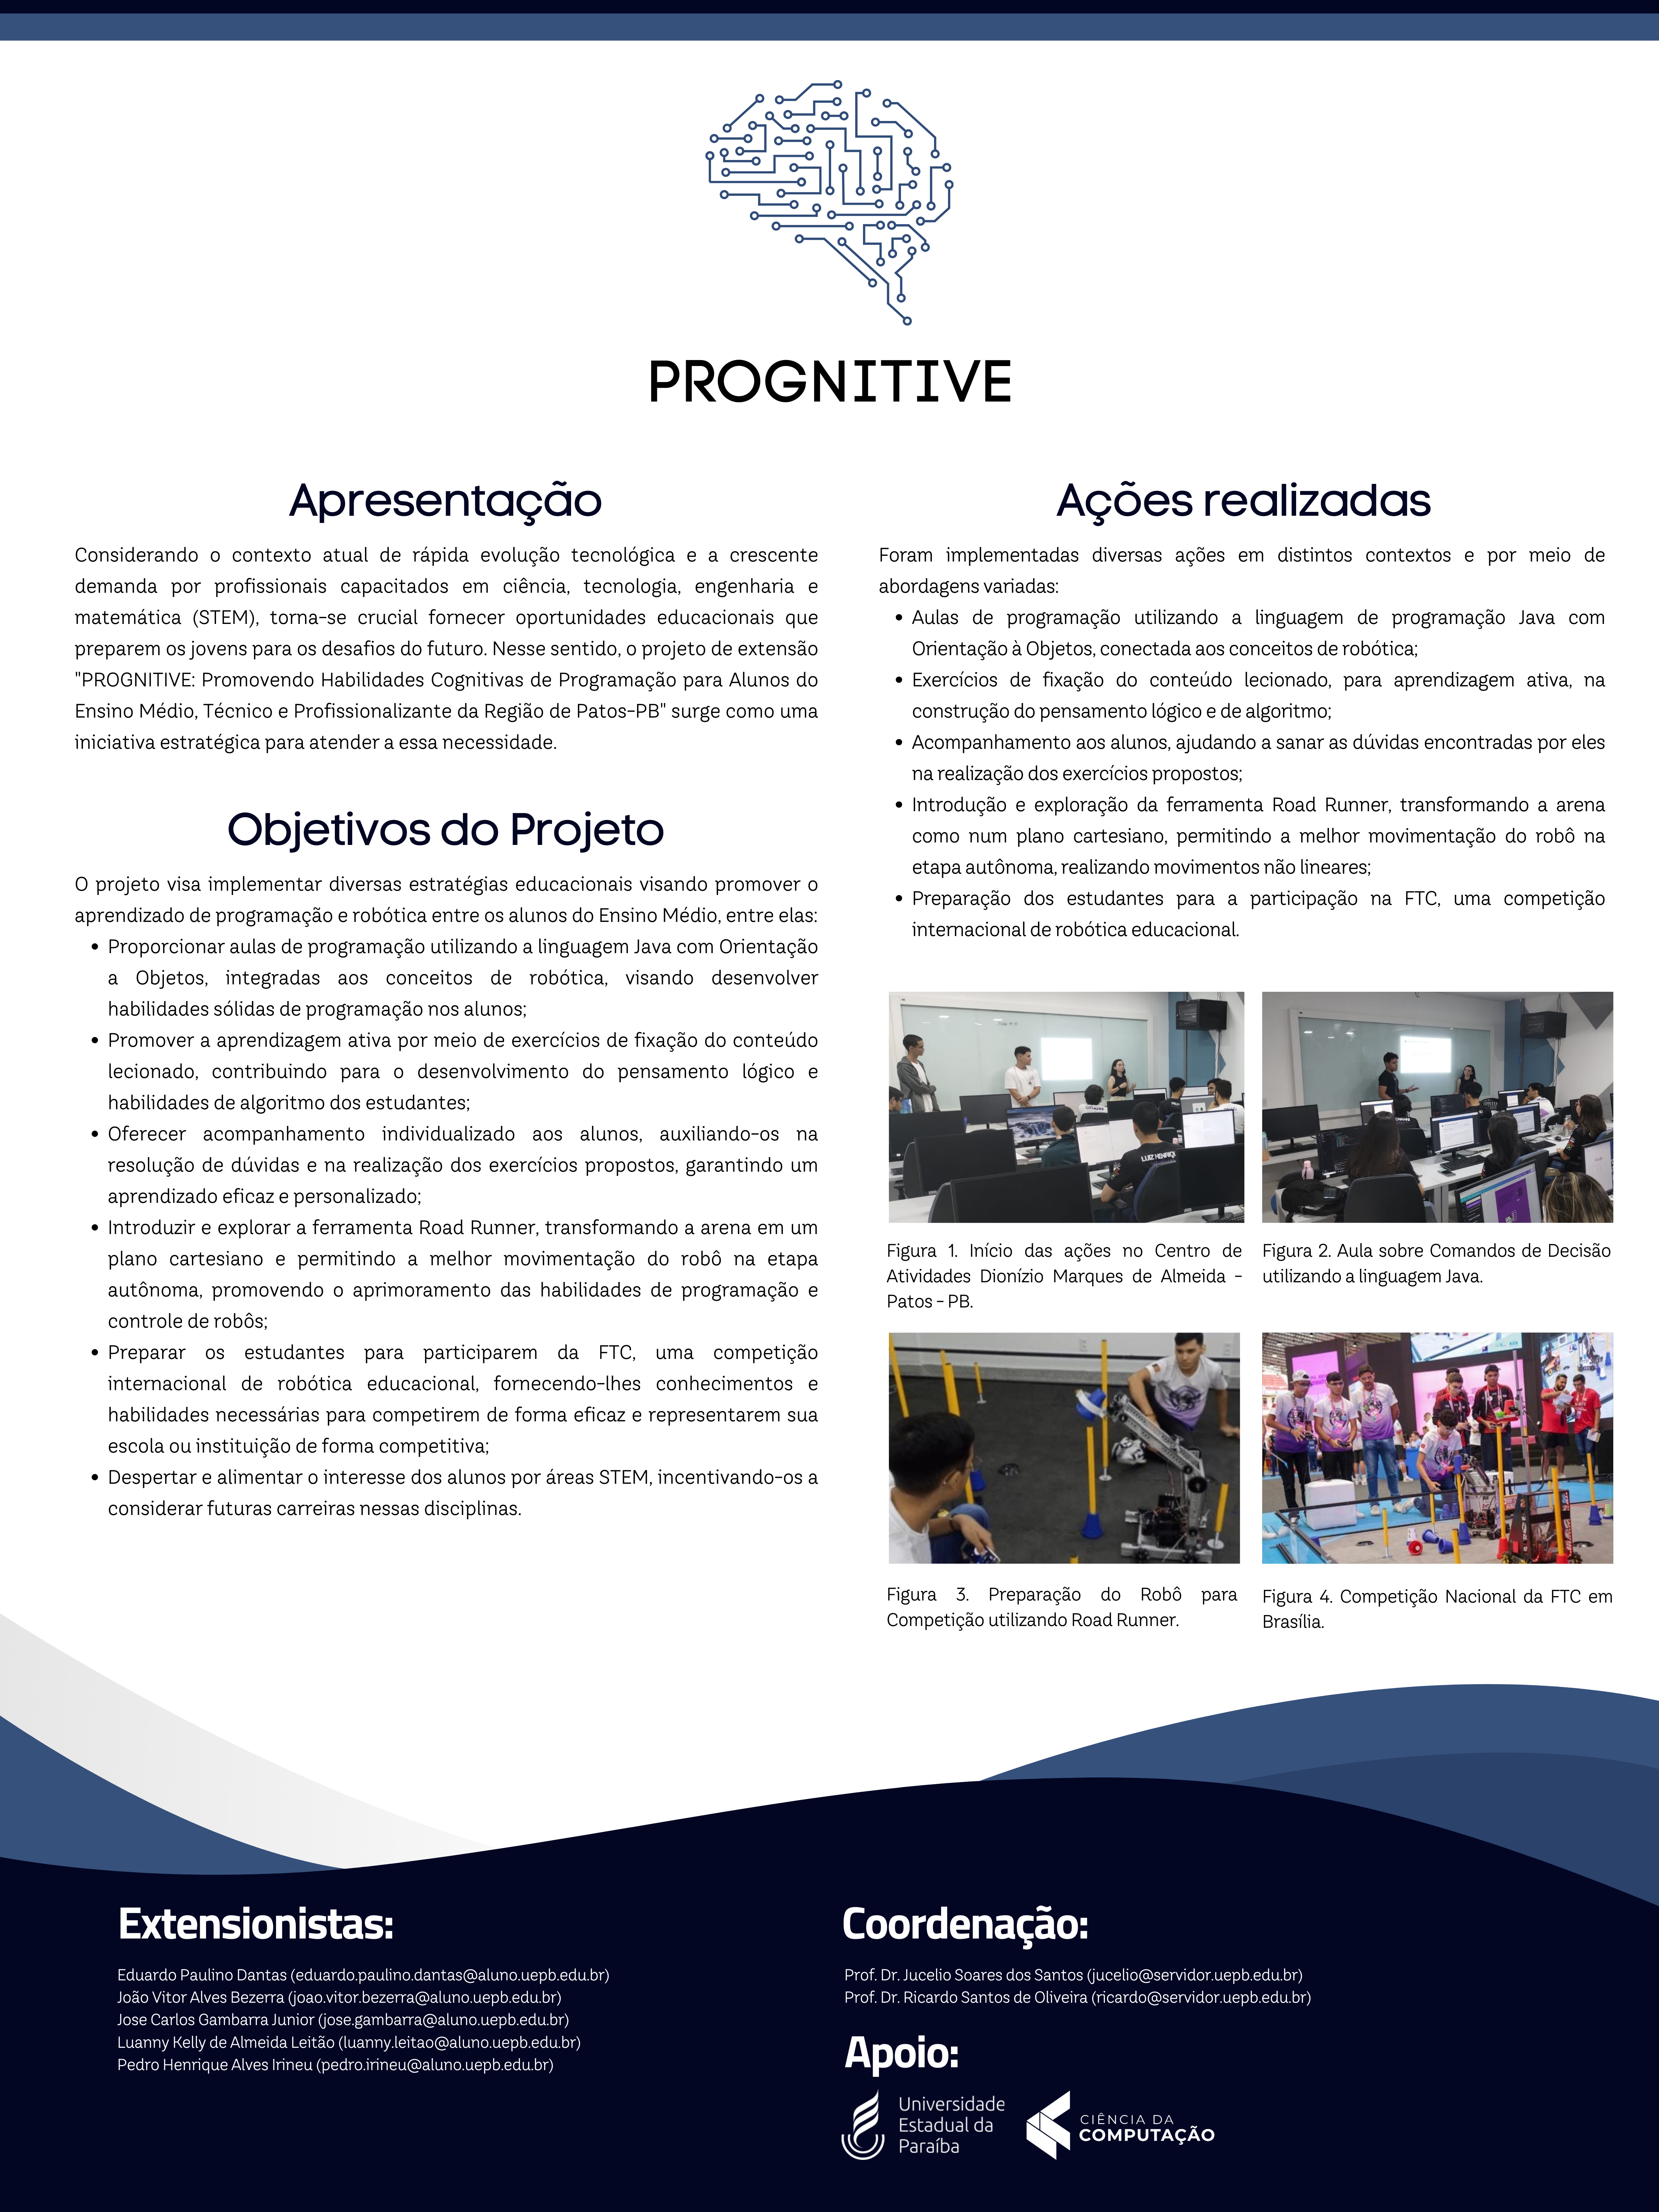
\includegraphics[scale=0.08]{imagens/imagem13.png}
    \includegraphics[scale=0.2125]{imagens/imagem12.jpeg}
\end{figure}

Essas atividades de extensão não apenas contribuíram para a disseminação do conhecimento em computação e robótica, mas também fortaleceram os laços entre a universidade e a comunidade externa. Ao participar de eventos como o VI Semana Zero do Curso de Computação, o I Congresso de Fluência entre Ensino, Tecnologia e Gestão, e a VII Semana Zero do Curso de Computação, conseguimos estabelecer conexões valiosas com estudantes, professores e pesquisadores, ampliando a visibilidade do projeto e atraindo novos colaboradores. Essas iniciativas tiveram um impacto significativo na promoção da educação em ciências exatas e tecnologia, além de proporcionar um ambiente de troca de conhecimentos e experiências.
\chapter{OUTRAS ATIVIDADES DE EXTENSÃO REALIZADAS}

Durante o período do projeto, não foram realizadas outras atividades além das mencionadas anteriormente. No entanto, estamos abertos a futuras oportunidades de realizar atividades como monografias, produção de livros, revistas, artigos e outros projetos que possam contribuir para a disseminação do conhecimento e fortalecimento das relações com a comunidade.



%referências
\bibliography{modelo_Bibtex}

\phantompart
\printindex

\end{document}